\documentclass[12pt, twoside]{article}
\input{../preamble}

\fancyhead[LE]{\thepage}
\fancyhead[RO]{\thepage}
\fancyhead[LO]{La Scuola d'Italia / Dr.\ Huson / IB Math: Probability --- Solutions \\* 11 March 2026}

\begin{document}
\subsubsection*{4.18 Homework: Probability Review --- Solutions}

\begin{enumerate}[itemsep=0.15cm]

%--- Problem 1: Venn diagram ---
\item In a class of 30 students, some study Spanish ($S$) and some study French ($F$).
Five students study both languages.

\begin{center}
\vspace{-0.2cm}
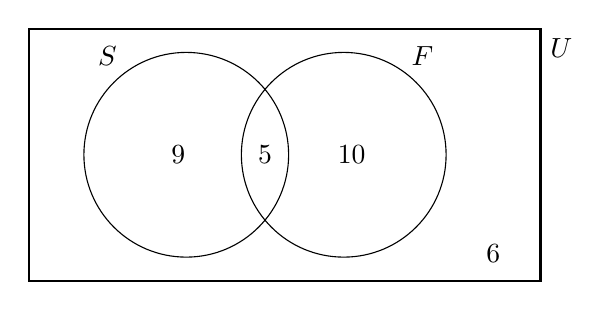
\begin{tikzpicture}
  \draw[thick] (0,0) rectangle (6.5,3.2);
  \node[anchor=north west] at (6.5,3.2) {$U$};
  \draw (2.0,1.6) circle (1.3cm);
  \node at (1.0,2.85) {$S$};
  \draw (4.0,1.6) circle (1.3cm);
  \node at (5.0,2.85) {$F$};
  \node at (1.9,1.6) {$9$};
  \node at (3.0,1.6) {$5$};
  \node at (4.1,1.6) {$10$};
  \node at (5.9,0.35) {$6$};
\end{tikzpicture}
\vspace{-0.2cm}
\end{center}

\begin{enumerate}[itemsep=0.1cm]
  \item Write down the number of students who study Spanish. \hfill [1]
  \item One student is chosen at random. Find the probability that
  \begin{enumerate}[label=(\roman*), itemsep=0.1cm]
    \item the student does not study Spanish; \hfill [1]
    \item the student studies Spanish or French, but not both. \hfill [2]
  \end{enumerate}
\end{enumerate}

\vfill

\begin{tikzpicture}
  \draw (0,0) rectangle (15.5,6);
  \node[anchor=north west, inner sep=0.40cm] at (0,6) {%
    \begin{minipage}[t]{14.7cm}%
      \textbf{Solutions}\\[0.4cm]
      \textbf{(a)}\enspace $n(S) = 9 + 5 = \mathbf{14}$\\[0.4cm]
      \textbf{(b)(i)}\enspace $\mathrm{P}(S') = \dfrac{10 + 6}{30} = \dfrac{16}{30} = \mathbf{\dfrac{8}{15}}$\\[0.4cm]
      \textbf{(b)(ii)}\enspace Spanish or French but not both $= 9 + 10 = 19$\\[0.1cm]
      \hspace*{2.5em}$\mathrm{P} = \dfrac{19}{30}$%
    \end{minipage}%
  };
\end{tikzpicture}

%--- Problem 2: Mutually exclusive ---
\item Events $C$ and $D$ are mutually exclusive with
$\mathrm{P}(C) = 0.35$ and $\mathrm{P}(D) = 0.25$.

\begin{enumerate}[itemsep=0.1cm]
  \item Write down $\mathrm{P}(C \cap D)$. \hfill [1]
  \item Find $\mathrm{P}(C \cup D)$. \hfill [2]
\end{enumerate}

\vfill

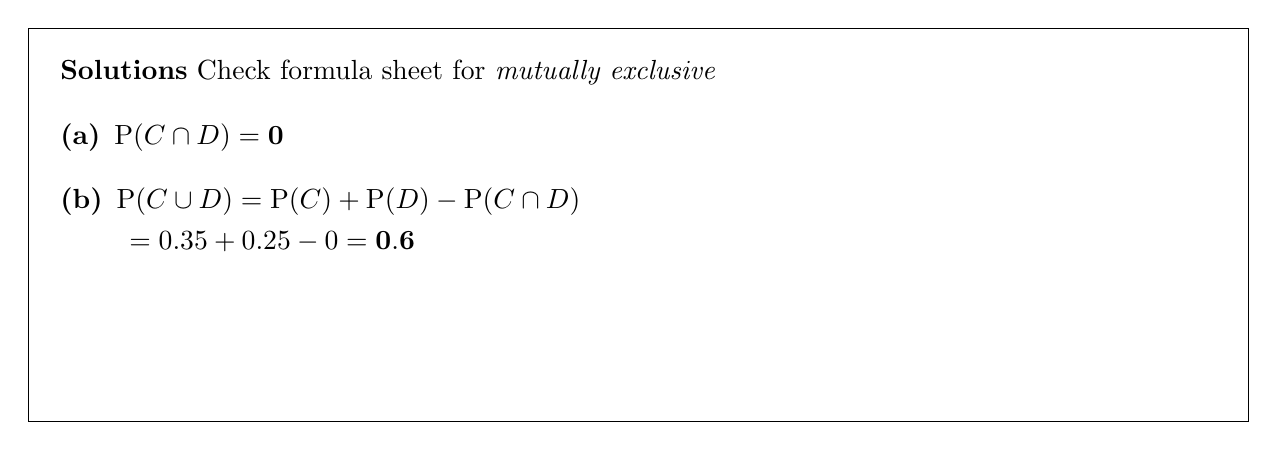
\begin{tikzpicture}
  \draw (0,0) rectangle (15.5,5);
  \node[anchor=north west, inner sep=0.40cm] at (0,5) {%
    \begin{minipage}[t]{14.7cm}%
      \textbf{Solutions} Check formula sheet for \emph{mutually exclusive} \\[0.4cm]
      \textbf{(a)}\enspace $\mathrm{P}(C \cap D) = \mathbf{0}$\\[0.4cm]
      \textbf{(b)}\enspace $\mathrm{P}(C \cup D) = \mathrm{P}(C) + \mathrm{P}(D) - \mathrm{P}(C \cap D)$\\[0.1cm]
      \hspace*{2.5em}$= 0.35 + 0.25 - 0 = \mathbf{0.6}$%
    \end{minipage}%
  };
\end{tikzpicture}

\newpage
%--- Problem 3: Venn with unknowns ---
\item In a group of 40 people, 22 like tea and 15 like coffee.
Eight people like both, as shown in the Venn diagram.
The values $\boldsymbol{a}$ and $\boldsymbol{b}$ represent numbers of people.

\begin{center}
\vspace{-0.2cm}
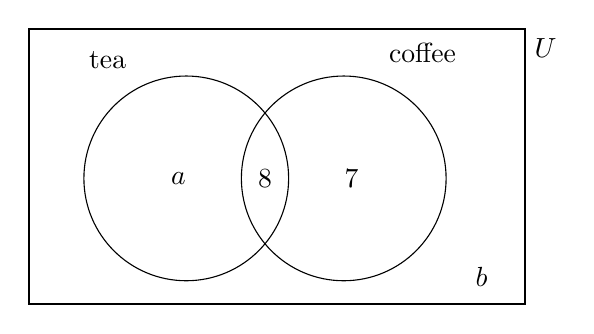
\begin{tikzpicture}
  \draw[thick] (0,0) rectangle (6.3,3.5);
  \node[anchor=north west] at (6.3,3.5) {$U$};
  \draw (2.0,1.6) circle (1.3cm);
  \node at (1,3.1) {tea};
  \draw (4.0,1.6) circle (1.3cm);
  \node at (5,3.2) {coffee};
  \node at (1.9,1.6) {$a$};
  \node at (3.0,1.6) {$8$};
  \node at (4.1,1.6) {$7$};
  \node at (5.75,0.35) {$b$};
\end{tikzpicture}
\vspace{-0.2cm}
\end{center}

\begin{enumerate}[itemsep=0.0cm]
  \item Find the value of $a$. \hfill [1]
  \item Find the value of $b$. \hfill [1]
  \item A person is chosen at random. Find the probability that the person
        likes coffee but not tea. \hfill [1]
  \item Find the probability that a person likes tea given that they like coffee. \hfill [2]
\end{enumerate}


\begin{tikzpicture}
  \draw (0,0) rectangle (15.5,7);
  \node[anchor=north west, inner sep=0.40cm] at (0,7) {%
    \begin{minipage}[t]{14.7cm}%
      \textbf{Solutions}\\[0.4cm]
      \textbf{(a)}\enspace $a + 8 = 22 \;\Rightarrow\; a = \mathbf{14}$\\[0.4cm]
      \textbf{(b)}\enspace $14 + 8 + 7 + b = 40 \;\Rightarrow\; b = \mathbf{11}$\\[0.4cm]
      \textbf{(c)}\enspace Coffee but not tea is the ``coffee only'' region $= 7$\\[0.1cm]
      \hspace*{2.5em}$\mathrm{P}(\text{coffee} \cap \text{tea}') = \dfrac{7}{40}$\\[0.4cm]
      \textbf{(d)}\enspace $\mathrm{P}(\text{tea} \mid \text{coffee})
        = \dfrac{\mathrm{P}(\text{tea} \cap \text{coffee})}{\mathrm{P}(\text{coffee})}
        = \dfrac{8/40}{15/40} = \dfrac{8}{15}$%
    \end{minipage}%
  };
\end{tikzpicture}

\newpage
%--- Problem 4: Two-way table with independence test ---
\item The following table shows the travel method and punctuality of 20 students.

\renewcommand{\arraystretch}{1.6}
\begin{center}
\begin{tabular}{|r|c|c|c|}
    \hline
    & Punctual ($P$) & Sometimes late ($T$) & Total \\
    \hline
    Walk    & 3  & 7 & 10 \\
    \hline
    Bus     & 2  & 8  & 10  \\
    \hline
    Total   & 5  & 15 & 20 \\
    \hline
\end{tabular}
\end{center}

\begin{enumerate}[itemsep=0.0cm]
  \item Find the probability that a randomly chosen student walks to school
        and is punctual. \hfill [1]
  \item Find $\mathrm{P}(\text{punctual} \mid \text{bus})$. \hfill [2]
  \item Determine whether ``walks to school'' and ``is punctual'' are independent events.
        Show your working and justify your answer. \hfill [3]
\end{enumerate}


\begin{tikzpicture}
  \draw (0,0) rectangle (15.5,8);
  \node[anchor=north west, inner sep=0.40cm] at (0,8) {%
    \begin{minipage}[t]{14.7cm}%
      \textbf{Solutions}\\[0.4cm]
      \textbf{(a)}\enspace $\mathrm{P}(W \cap P) = \dfrac{3}{20}$\\[0.4cm]
      \textbf{(b)}\enspace $\mathrm{P}(P \mid B)
        = \dfrac{\mathrm{P}(P \cap B)}{\mathrm{P}(B)}
        = \dfrac{2/20}{10/20} = \dfrac{2}{10}$\\[0.4cm]
      \textbf{(c)}\enspace If independent, then $\mathrm{P}(W \cap P) = \mathrm{P}(W) \times \mathrm{P}(P)$\\[0.2cm]
      \hspace*{2.5em}$\mathrm{P}(W) \times \mathrm{P}(P)
        = 0.5 \times 0.25
        = 0.125$\\[0.2cm]
      \hspace*{2.5em}$\mathrm{P}(W \cap P) = \dfrac{3}{20} = 0.15$\\[0.2cm]
      \hspace*{2.5em}$0.15 \neq 0.125$, so the events are \textbf{not independent}.%
    \end{minipage}%
  };
\end{tikzpicture}


\newpage
%--- Problem 5: Tree diagram ---
\item A bakery makes bread using two ovens. Oven $A$ bakes $70\%$ of the loaves
and oven $B$ bakes the remaining $30\%$. The probability that a loaf from
oven $A$ is burnt is $0.04$. The probability that a loaf from oven $B$ is burnt
is $0.10$.

\begin{enumerate}[itemsep=0.3cm]
  \item Complete the tree diagram below, showing all probabilities. \hfill [3]

  \begin{center}
  \begin{tikzpicture}
    % Main branches
    \draw (0,0) -- (3.5, 2.0);
    \draw (0,0) -- (3.5,-2.0);
    % Oven A branches
    \draw (3.5, 2.0) -- (7.0, 3.2);
    \draw (3.5, 2.0) -- (7.0, 1.3);
    % Oven B branches
    \draw (3.5,-2.0) -- (7.0,-1.3);
    \draw (3.5,-2.0) -- (7.0,-3.2);
    % First-level labels
    \node[above] at (1.75, 1.0) {$0.7$};
    \node[below] at (1.75,-1.0) {$0.3$};
    \node[above left] at (3.5, 2.0) {\small Oven $A$};
    \node[below left] at (3.5,-2.0) {\small Oven $B$};
    % Second-level labels (filled in)
    \node[above] at (5.25, 2.6) {$0.04$};
    \node[below] at (5.25, 0.8) {$0.96$};
    \node[above] at (5.25,-1.65) {$0.10$};
    \node[below] at (5.25,-3.5) {$0.90$};
    % Outcome labels
    \node[anchor=west] at (7.15, 3.2) {Burnt};
    \node[anchor=west] at (7.15, 1.3) {Not burnt};
    \node[anchor=west] at (7.15,-1.3) {Burnt};
    \node[anchor=west] at (7.15,-3.2) {Not burnt};
    % Composite probabilities (filled in)
    \node[anchor=west] at (10.0, 3.2) {$= 0.028$};
    \node[anchor=west] at (10.0, 1.3) {$= 0.672$};
    \node[anchor=west] at (10.0,-1.3) {$= 0.030$};
    \node[anchor=west] at (10.0,-3.2) {$= 0.270$};
  \end{tikzpicture}
  \end{center}

  \item A loaf is selected at random. Find the probability that the loaf is
  \begin{enumerate}[label=(\roman*), itemsep=0.1cm]
    \item burnt and from oven $A$; \hfill [2]
    \item burnt. \hfill [2]
  \end{enumerate}

  \item Given that a loaf is burnt, find the probability that it came from
        oven $A$. \hfill [3]
\end{enumerate}

\begin{tikzpicture}
  \draw (0,0) rectangle (15.5,7);
  \node[anchor=north west, inner sep=0.40cm] at (0,7) {%
    \begin{minipage}[t]{14.7cm}%
      \textbf{Solutions}\\[0.4cm]
      \textbf{(a)}\enspace Blanks: $1 - 0.04 = 0.96$; \enspace $0.10$; \enspace $1 - 0.10 = 0.90$\\[0.1cm]
      \hspace*{2.5em}Composite: $0.7 \times 0.04 = 0.028$; \enspace
        $0.7 \times 0.96 = 0.672$\\[0.1cm]
      \hspace*{2.5em}\phantom{Composite: }$0.3 \times 0.10 = 0.030$; \enspace
        $0.3 \times 0.90 = 0.270$\\[0.4cm]
      \textbf{(b)(i)}\enspace $\mathrm{P}(A \cap \text{Burnt}) = 0.7 \times 0.04 = \mathbf{0.028}$\\[0.4cm]
      \textbf{(b)(ii)}\enspace $\mathrm{P}(\text{Burnt}) = 0.028 + 0.030 = \mathbf{0.058}$\\[0.4cm]
      \textbf{(c)}\enspace $\mathrm{P}(A \mid \text{Burnt})
        = \dfrac{\mathrm{P}(A \cap \text{Burnt})}{\mathrm{P}(\text{Burnt})}
        = \dfrac{0.028}{0.058} = 0.48275 \ldots \approx \mathbf{0.483}$%
    \end{minipage}%
  };
\end{tikzpicture}

\newpage
%--- Problem 6: Without replacement ---
\item A bag contains 5 red marbles and 7 blue marbles. Two marbles are
drawn at random, one after the other, without replacement.

\begin{enumerate}[itemsep=0.1cm]
  \item Find the probability that both marbles are red. \hfill [2]
  \item Find the probability that both marbles are the same colour. \hfill [3]
  \item Find the probability that both marbles are red given that
        at least one marble is red. \hfill [3]
\end{enumerate}

\emph{A tree is a good way to organize these two-step problems.}

\begin{center}
\begin{tikzpicture}[scale=0.9]
  % First draw
  \draw (0,0) -- (3.5, 2.0);
  \draw (0,0) -- (3.5,-2.0);
  % Second draw — from Red
  \draw (3.5, 2.0) -- (7.0, 3.2);
  \draw (3.5, 2.0) -- (7.0, 1.3);
  % Second draw — from Blue
  \draw (3.5,-2.0) -- (7.0,-1.3);
  \draw (3.5,-2.0) -- (7.0,-3.2);
  % First-level labels
  \node[above] at (1.75, 1.0) {$\frac{5}{12}$};
  \node[below] at (1.75,-1.0) {$\frac{7}{12}$};
  \node[above left] at (3.5, 2.0) {\small R};
  \node[below left] at (3.5,-2.0) {\small B};
  % Second-level labels
  \node[above] at (5.25, 2.6) {$\frac{4}{11}$};
  \node[below] at (5.25, 1.7) {$\frac{7}{11}$};
  \node[above] at (5.25,-1.65) {$\frac{5}{11}$};
  \node[below] at (5.25,-2.9) {$\frac{6}{11}$};
  % Outcome labels
  \node[anchor=west] at (7.15, 3.2) {RR};
  \node[anchor=west] at (7.15, 1.3) {RB};
  \node[anchor=west] at (7.15,-1.3) {BR};
  \node[anchor=west] at (7.15,-3.2) {BB};
  % Composite probabilities
  \node[anchor=west] at (9.0, 3.2) {$= \frac{20}{132}$};
  \node[anchor=west] at (9.0, 1.3) {$= \frac{35}{132}$};
  \node[anchor=west] at (9.0,-1.3) {$= \frac{35}{132}$};
  \node[anchor=west] at (9.0,-3.2) {$= \frac{42}{132}$};
\end{tikzpicture}
\end{center}

\begin{tikzpicture}
  \draw (0,0) rectangle (15.5,9);
  \node[anchor=north west, inner sep=0.40cm] at (0,9) {%
    \begin{minipage}[t]{14.7cm}%
      \textbf{Solutions}\\[0.4cm]
      \textbf{(a)}\enspace $\mathrm{P}(RR) = \dfrac{5}{12} \times \dfrac{4}{11}
        = \dfrac{20}{132} = \dfrac{5}{33}$\\[0.5cm]
      \textbf{(b)}\enspace $\mathrm{P}(BB) = \dfrac{7}{12} \times \dfrac{6}{11}
        = \dfrac{42}{132} = \dfrac{7}{22}$\\[0.3cm]
      \hspace*{2.5em}$\mathrm{P}(\text{same}) = \mathrm{P}(RR) + \mathrm{P}(BB)
        = \dfrac{20}{132} + \dfrac{42}{132}
        = \dfrac{62}{132} = \dfrac{31}{66}$\\[0.5cm]
      \textbf{(c)}\enspace $\mathrm{P}(RR \mid \text{at least one } R)
        = \dfrac{\mathrm{P}(RR)}{\mathrm{P}(\text{at least one } R)}$\\[0.3cm]
      \hspace*{2.5em}$\mathrm{P}(\text{at least one } R)
        = 1 - \mathrm{P}(BB)
        = 1 - \dfrac{42}{132}
        = \dfrac{90}{132}$\\[0.3cm]
      \hspace*{2.5em}$\mathrm{P}(RR \mid \text{at least one } R)
        = \dfrac{20/132}{90/132}
        = \dfrac{20}{90} = \dfrac{2}{9}$%
    \end{minipage}%
  };
\end{tikzpicture}

\end{enumerate}
\end{document}
